% (C) Copyright 2016
% Urs Fässler, www.bitzgi.ch
% SPDX-License-Identifier: CC-BY-SA-4.0

\usepackage[utf8x]{inputenc}
\usepackage{ucs}
\usepackage{amsmath}
\usepackage{amsfonts}
\usepackage{amssymb}
\usepackage{graphicx}
\usepackage{appendixnumberbeamer}
\usepackage{url}
\usepackage{makecell}
\usepackage{svgcolor}
\usepackage{tikz}
\usetikzlibrary{arrows, positioning, shapes}
\usetikzlibrary{backgrounds, fit, decorations.pathreplacing, calc}
\usepackage{multicol}

\title{GPL, MIT, ..., WTF?}
\subtitle{Freie Software Lizenzen}
\author{Urs Fässler}
\date{9.2.2017}
\institute
{
	FSFE Lokalgruppe Zürich Meeting
}
\subject{CC-BY-SA Urs Fässler}

\newcommand{\todo}[1]{{\color{red}TODO: #1}}

\newcommand{\hnote}[1]{\only<handout>{\footnote{#1}}}
\newcommand{\hcite}[1]{\only<handout>{\cite{#1}}}

\newcommand*\oldmacro{}%
\let\oldmacro\insertshorttitle%
\renewcommand*\insertshorttitle{%
	\oldmacro\hfill%
	\insertframenumber
}
\usetheme{Luebeck}

% remove navigation bars
\beamertemplatenavigationsymbolsempty

% remove section information
\setbeamertemplate{headline}{}

\newcommand{\subsectionframe}
{
	\begin{frame}[noframenumbering]
		\begin{center}
			\begin{huge}
				\insertsubsection
			\end{huge}
		\end{center}
	\end{frame}
}

% Table formatting
\renewcommand\theadalign{cb}
\renewcommand\theadfont{\bfseries}
\renewcommand\theadgape{\Gape[4pt]}
\renewcommand\cellgape{\Gape[4pt]}


\begin{document}

\titlepage

\section{Teaser}
\begin{frame}
	\begin{itemize}
		\item eigenes Foto, darf es kopiert und verwendet werden?
		\item ändert das Copyright Zeichen und Name etwas?
		\item ändert ein CC-BY-SA etwas?
	\end{itemize}
\end{frame}

\section{Thema}
\note
{
	\begin{itemize}
		\item Eine Einführung in die Lizenzen der Freien Software (Open Source)
	\end{itemize}
}

\section{Behauptung}
\note
{
	\begin{itemize}
		\item Korrekte Verwendung Freier Software ist nicht schwer
	\end{itemize}
}

% (C) Copyright 2016
% Urs Fässler, www.bitzgi.ch
% SPDX-License-Identifier: CC-BY-SA-4.0

\section{Vorstellung}
\begin{frame}{About me}
	\begin{center}
		\begin{tikzpicture}
		[
			node distance = 3 cm,
			box/.style = {align=center},
		]
		
		\visible<1-> {
			\node[box] (me) {\large{Urs Fässler}};
		}
		
		\visible<2-> {
			\node[box, above left of = me] {
\includegraphics[height=1.25cm]{res/fellowship-page-logo.pdf}};
		}
	
		\visible<3-> {
			\node[box, above right of = me] {
\includegraphics[height=1.25cm]{res/bbv.pdf}};
		}
	
		\visible<4-> {
			\node[box, below right of = me] {
\includegraphics[height=1.5cm]{res/cpp.pdf}};
		}
	
		\visible<5-> {
			\node[box, below left of = me] {
\includegraphics[height=4cm]{res/gnu-and-penguin-color.png}};
		}
		\end{tikzpicture}
		\hspace*{1cm}
	\end{center}
\end{frame}
\note
{
	\begin{itemize}
		\item Urs Fässler
		\item Aktiv in der FSFE Lokalgruppe Zürich
		\item Senior Embedded Software Ingenieur @ bbv Software Service \url{http://bbv.ch}
		\item Entwickeln von Software
		\item Erstellen von Systemen auf Basis GNU/Linux
		\item FSFE Fellow: \url{https://fsfe.org/contribute/getyourgraphic.en.html}
		\item Gnu-and-penguin-color.png: GFDL 1.2+ or CC-BY-SA 3.0 (\url{https://commons.wikimedia.org/wiki/File:Gnu-and-penguin-color.png})
	\end{itemize}
}

\begin{frame}{Haftungsausschluss}
	\begin{itemize}
		\item Dieser Vortrag ist keine Rechtsberatung.
		\item Für eine Rechtsberatung konsultieren Sie bitte einen Anwalt.
	\end{itemize}
\end{frame}

\section{Inhalt}

\begin{frame}{Inhalt}
	\begin{itemize}
		\item \nameref{sec:voraussetzungen}
		\item \nameref{sec:lizenzen}
		\item \nameref{sec:handhabung}
		\item \nameref{sec:zusammenfassung}
	\end{itemize}
\end{frame}

% (C) Copyright 2016
% Urs Fässler, www.bitzgi.ch
% SPDX-License-Identifier: CC-BY-SA-4.0

\subsection{Grundlagen}
\label{sec:voraussetzungen}
\subsectionframe

\begin{frame}{Freie Software}
	\todo{Farben, kanten abrunden}
	\begin{center}
		\begin{tikzpicture}
		[
			node distance = 2 cm,
			box/.style = {thick, draw=black, fill=red, align=center, inner sep = 0.3cm},
		]
		
		\visible<1-> {
			\node[box] (freedom) {Die Freiheit zu};
		}
		
		\visible<2-> {
			\node[box, above left of = freedom] {Verwenden\only<handout>{\\Die Freiheit, die Software uneingeschränkt und für jeden Zweck einzusetzen.}};
		}
	
		\visible<3-> {
			\node[box, above right of = freedom] {Verstehen\only<handout>{\\Die Freiheit, die Funktionsweise der Software untersuchen und verstehen zu können.}};
		}
	
		\visible<4-> {
			\node[box, below left of = freedom] {Verbreiten\only<handout>{\\Die Freiheit, Kopien der Software zu verbreiten, um damit seinen Mitmenschen zu helfen.}};
		}
	
		\visible<5-> {
			\node[box, below right of = freedom] {Verbessern\only<handout>{\\Die Freiheit, die Software zu verbessern und die Verbesserungen an die Öffentlichkeit weiterzugeben, sodass die gesamte Gesellschaft davon profitieren kann.}};
		}
	
		\end{tikzpicture}
	\end{center}
\end{frame}
\note
{
	\url{http://www.inf-schule.de/software/freie\_software/02\_freiheiten\_freier\_software}
}

\begin{frame}{Frei und Kommerziell}
	\begin{center}
		\begin{tabular}{c|c|c|}
			 & \thead{proprietär} &  \thead{frei} \\ 
			\hline 
			\thead{kommerziell} & \makecell{Windows\\Mac OS} & \makecell{Red Hat Enterprise\\Linux (RHEL)}\\ 
			\hline 
			\thead{gratis} & \makecell{(iOS)\\Freeware} & \makecell{Debian} \\ 
			\hline 
		\end{tabular} 
	\end{center}
\end{frame}

\begin{frame}{Intellectual Property (IP)}
	\begin{center}
		Geistiges Eigentum
		\begin{tabular}{ccc}
		\hspace{3cm} & \hspace{3cm} & \hspace{3cm} \\
		Patent & Markenrecht & Urheberrecht \\ 
		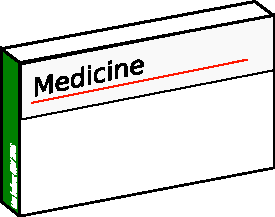
\includegraphics[height=2cm]{res/tulipan-Pharmaceutical-carton.pdf} & 
\includegraphics[height=2.5cm]{res/gnu-head.pdf} & 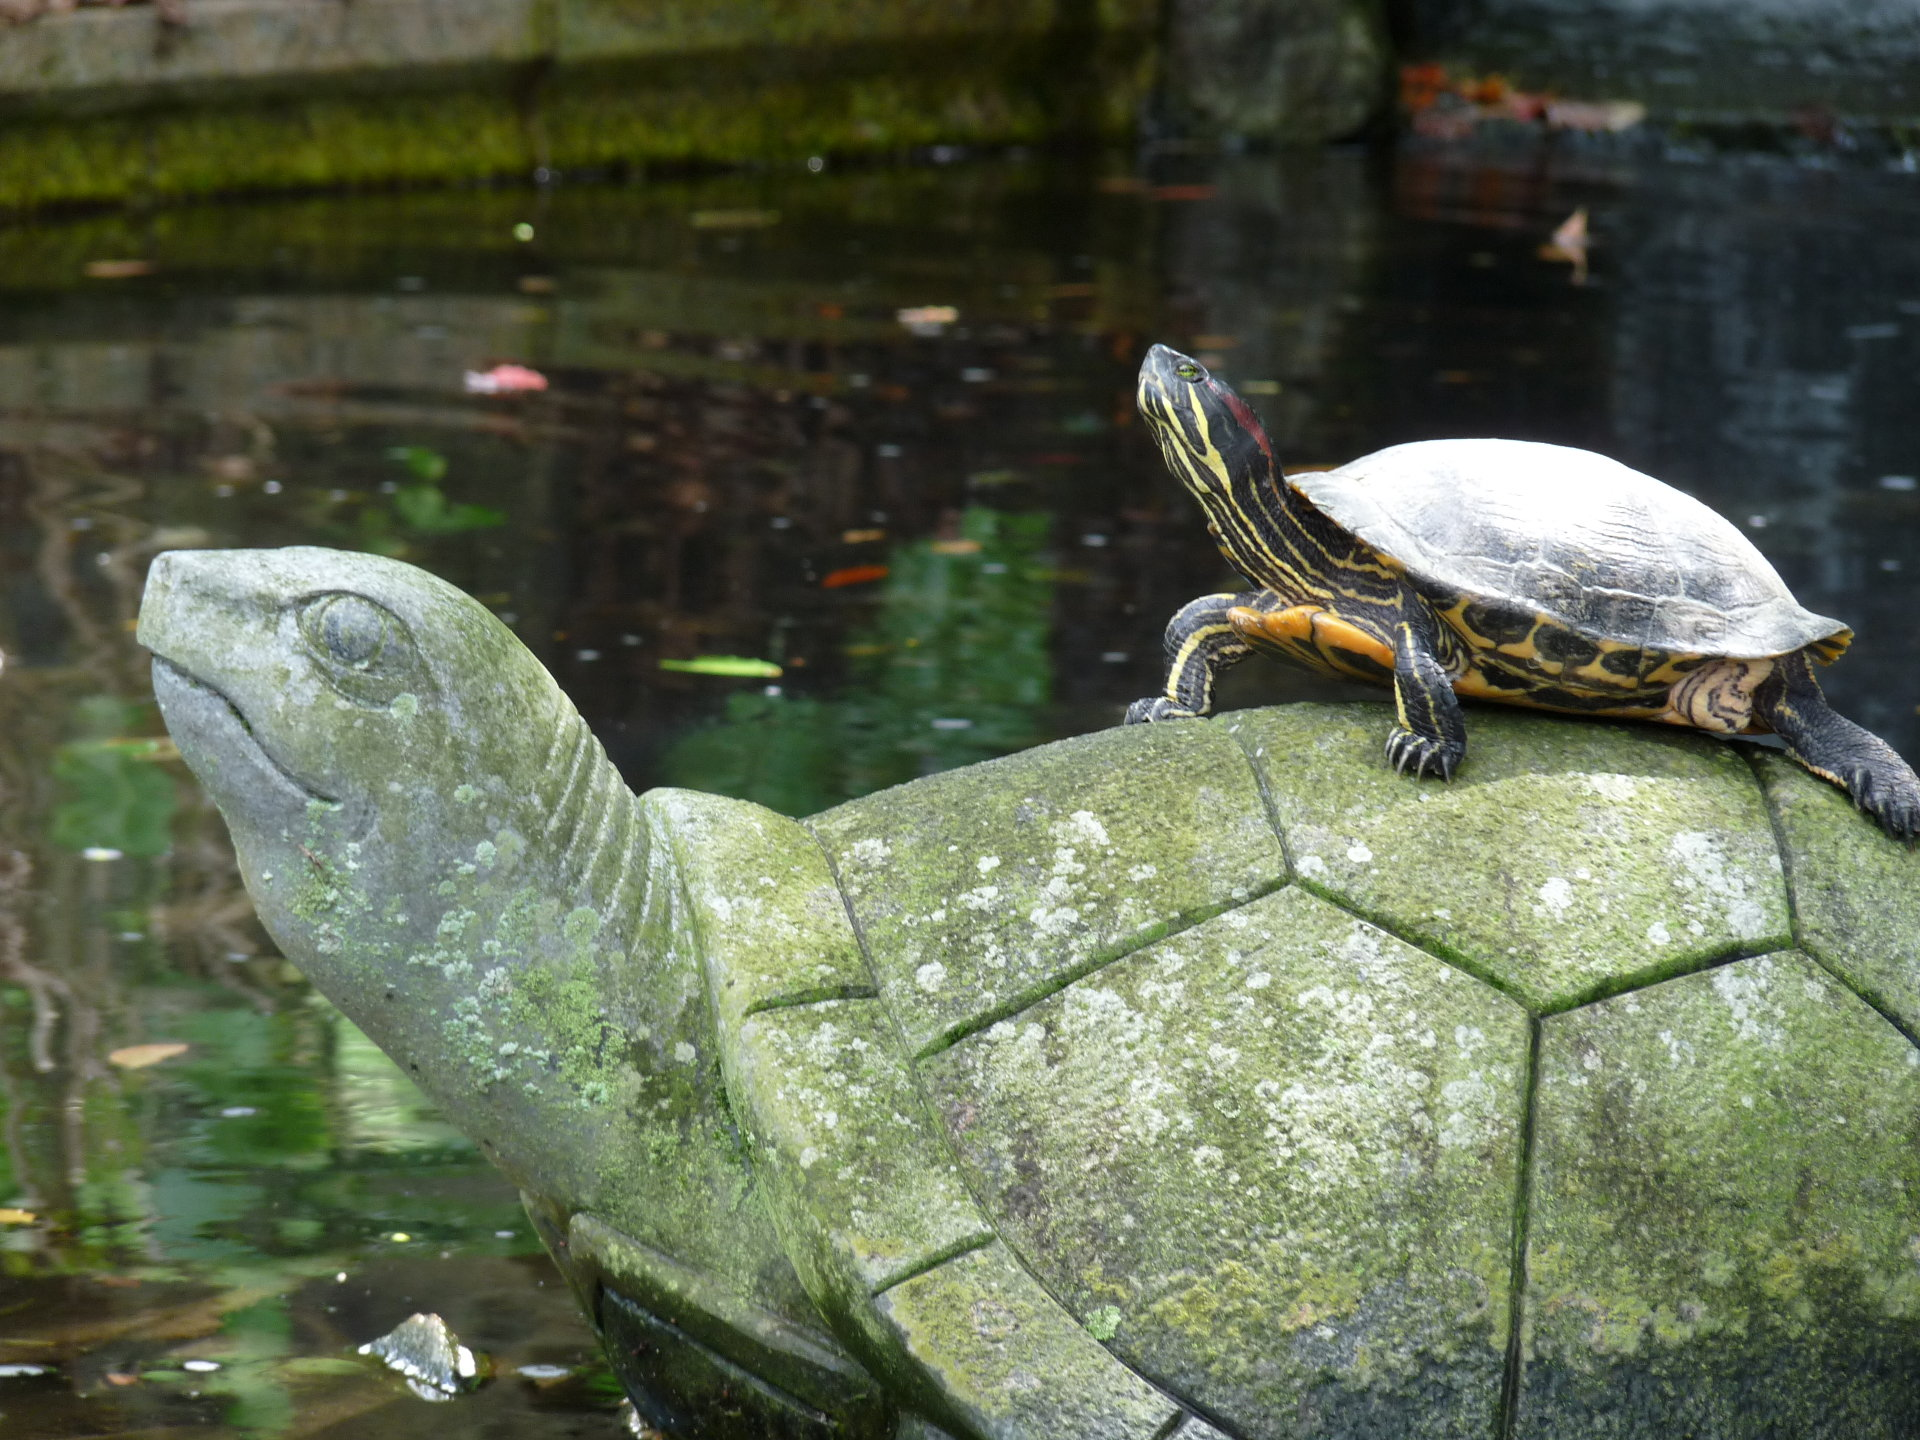
\includegraphics[height=2.5cm]{res/turtles.jpg} \\ 
		\only<handout>
		{
			Auf Antrag & Auf Antrag & automatisch \\
			\makecell{Schutz der\\Investition} & \makecell{Schutz von\\Erkennungsmerkmal} & \makecell{Verwertungsrecht\\künstlerischer\\Schöpfungen} \\
			20 Jahre & beliebig erneuerbar & 70 Jahre nach Tod \\
		}
		\end{tabular} 
	\end{center}
\end{frame}
\note
{
	(IP, Intellectual Property, Geistiges Eigentum) \url{https://de.wikipedia.org/wiki/Geistiges\_Eigentum\#Systematik}
	\begin{itemize}
		\item Patent
		\begin{itemize}
			\item \url{https://de.wikipedia.org/wiki/Patent}
			\item Defensivpublikation
			\item Acarton with pills: CC-0 by tulipan \url{https://openclipart.org/detail/6135/pharmaceutical-carton}
		\end{itemize}
		\item Markenrecht
		\begin{itemize}
			\item \url{https://de.wikipedia.org/wiki/Marke_(Recht)}
			\item Firefox und Debian (Iceweasel): \url{https://lwn.net/Articles/676799/}
			\item A GNU Head: CC-BY-SA Etienne Suvasa; Trademark of the GNU Project: \url{https://www.gnu.org/graphics/agnuhead.html}
		\end{itemize}
		\item Urheberrecht
		\begin{itemize}
			\item \url{https://de.wikipedia.org/wiki/Urheberrecht}
			\item für Werke
			\item daher auch für Software
			\item gilt automatisch: \url{https://anwalt-im-netz.de/urheberrecht/urheberrecht-faq.html\#wann}
			\item Copyrightzeichen ist nicht nötig: \url{https://de.wikipedia.org/wiki/Copyrightzeichen}
			\item Nicht verzichtbar (kein public domain, Gemeinfreiheit: \url{https://de.wikipedia.org/wiki/Gemeinfreiheit\#Entlassung\_in\_die\_Gemeinfreiheit})
		\end{itemize}
	\end{itemize}
}

% (C) Copyright 2016
% Urs Fässler, www.bitzgi.ch
% SPDX-License-Identifier: CC-BY-SA-4.0

\subsection{Lizenzen}
\label{sec:lizenzen}
\subsectionframe

\begin{frame}{Lizenz-Kategorien}
	\begin{center}
		\begin{tabular}{ccc}
		\visible<2->{
\includegraphics[width=2.5cm]{res/PD-icon.pdf}} & \visible<4->{
\includegraphics[width=2.5cm]{res/by.pdf}} & \visible<3->{
\includegraphics[width=2.5cm]{res/copyleft.pdf}} \\ 
		\visible<2->{Public Domain} & \visible<4->{Permissiv} & \visible<3->{Copyleft} \\
		\hspace{3cm} & \hspace{3cm} & \hspace{3cm} \\
		\end{tabular} 
	\end{center}
\end{frame}
\note
{
	Public Domain Lizenzen
	\begin{itemize}
		\item nicht gültig in D-A-CH (\url{https://de.wikipedia.org/wiki/Gemeinfreiheit\#Public_Domain})
		\item Verwende CC-0
		\item CC-0: Public Domain (\url{https://creativecommons.org/about/downloads/})
	\end{itemize}
}
\note
{
	Permissive Lizenzen
	\begin{itemize}
		\item Darf
		\begin{itemize}
			\item Ist generell Freie Software
			\item Kommerzielle Verwendung
			\item Proprietäre Verwendung
		\end{itemize}
		\item Muss
		\begin{itemize}
			\item Copyright angeben
			\item Lizenz mitliefern
		\end{itemize}
	\end{itemize}
}
\note
{
	Copyleft Lizenzen \url{https://de.wikipedia.org/wiki/Copyleft}
	\begin{itemize}
		\item Darf
		\begin{itemize}
			\item Ist generell Freie Software
			\item Kommerzielle Verwendung
		\end{itemize}
		\item Darf nicht
		\begin{itemize}
			\item Proprietäre Verwendung
		\end{itemize}
		\item Muss
		\begin{itemize}
			\item Code veröffentlichen
			\item Copyright angeben
			\item Lizenz mitliefern
		\end{itemize}
	\end{itemize}
}

\begin{frame}{Kategorien Gegenüberstellung}
	\newcommand{\yes}{\makecell{\Large \color{green}\checkmark}}
	\newcommand{\no}{\makecell{\Large \boldmath \color{green}$\times$}}
	\newcommand{\dontknow}{\makecell{\Large \color{green}?}}
	\begin{tabular}{lccc}
		& \makecell{
\includegraphics[width=1cm]{res/PD-icon.pdf}\\Public Domain} & \makecell{
\includegraphics[width=1cm]{res/by.pdf}\\Permissiv} & \makecell{
\includegraphics[width=1cm]{res/copyleft.pdf}\\Copyleft} \\ 
		\hline
		\visible<2->{Freie Software} & \visible<3->{\yes & \yes & \yes} \\ 
		\hline 
		\visible<4->{Kommerziell} & \visible<5->{\yes & \yes & \yes} \\ 
		\hline 
		\visible<6->{Proprietär} & \visible<7->{\yes & \yes & \no} \\ 
		\hline 
		\visible<8->{Copyright angeben} & \visible<9->{\no & \yes & \yes} \\ 
		\hline 
		\visible<10->{Lizenz mitliefern} & \visible<11->{\no & \yes & \yes} \\ 
		\hline 
		\visible<12->{gültig in D-A-CH} & \visible<13->{\dontknow & \yes & \yes} \\
		\hline 
	\end{tabular} 
\end{frame}{

\begin{frame}{Public Domain Lizenzen}
	\begin{center}
		\pause
		
\includegraphics[width=3.5cm]{res/unlicense-logo.pdf}
		\hfill
		\pause
		
\includegraphics[height=3cm]{res/beer.pdf}
		\hfill
		\pause
		
\includegraphics[height=2.5cm]{res/WTFPL_logo.pdf}
		\\
		\vspace{1cm}
		\pause
		
\includegraphics[width=3cm]{res/cc-zero.pdf}
	\end{center}
\end{frame}
\note
{
	\begin{itemize}
		\item The Unlicense (\url{http://programmers.stackexchange.com/questions/147111/what-is-wrong-with-the-unlicense\#147120})
		\item Beer: CC-0 by drunken\_duck (\url{https://openclipart.org/detail/2214/beer})
		\item WTFPL (\url{https://en.wikipedia.org/wiki/WTFPL})
		\item An official logo for the WTFPL license: WTFPD by www.wtfpl.net \url{https://commons.wikimedia.org/wiki/File:WTFPL_logo.svg}
		\item CC-0: Public Domain (\url{https://creativecommons.org/about/downloads/})
	\end{itemize}
}

\begin{frame}{Permissive Lizenzen}
	\begin{center}
		\pause
		
\includegraphics[width=3.5cm]{res/mit-logo.pdf}
		\hfill
		\pause
		
\includegraphics[width=3.5cm]{res/bsd-logo.pdf}
		\hfill
		\pause
		
\includegraphics[width=3.5cm]{res/apache-logo.pdf}
		\\
		\vspace{1cm}
		\pause
		
\includegraphics[width=3cm]{res/cc-by.pdf}
	\end{center}
\end{frame}
\note
{
	\begin{itemize}
		\item MIT, BSD, Apache
		\item CC-BY: Public Domain (\url{https://creativecommons.org/about/downloads/})
	\end{itemize}
}

\begin{frame}{Copyleft Lizenzen}
	\begin{center}
		\pause
		
\includegraphics[height=1.5cm]{res/gpl-v3-logo.pdf}
		\hfill
		\pause
		
\includegraphics[height=1.5cm]{res/lgpl-v3-logo.pdf}
		\hfill
		\pause
		
\includegraphics[height=1.5cm]{res/agpl-v3-logo.pdf}
		\\
		\vspace{1cm}
		\pause
		
\includegraphics[width=3cm]{res/cc-by-sa.pdf}
	\end{center}
\end{frame}
\note
{
	\begin{itemize}
		\item GPL, LGPL, AGPL, MPL
		\item GPLv3 Logo: Public Domain by Free Software Foundation (\url{https://commons.wikimedia.org/wiki/File:GPLv3\_Logo.svg})
		\item LGPLv3 Logo: Public Domain by Free Software Foundation (\url{https://commons.wikimedia.org/wiki/File:LGPLv3\_Logo.svg})
		\item AGPLv3 Logo: Public Domain by Free Software Foundation (\url{https://commons.wikimedia.org/wiki/File:AGPLv3\_Logo.svg})
		\item CC-BY-SA: Public Domain (\url{https://creativecommons.org/about/downloads/})
	\end{itemize}
}

\begin{frame}{Detailliertere Informationen}
	\begin{itemize}
		\item \url{https://tldrlegal.com/}
	\end{itemize}
	\vspace{1em}
	\begin{center}
		\pause
		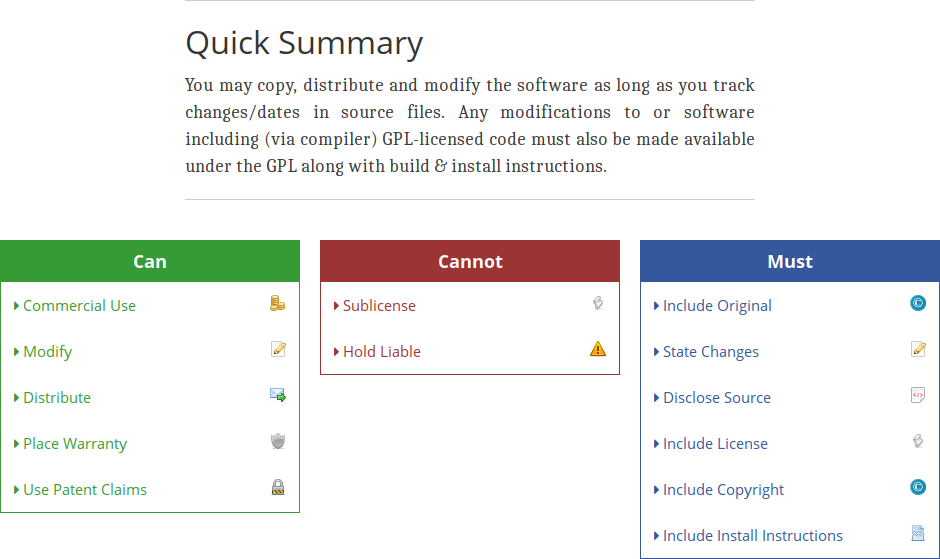
\includegraphics[height=5cm]{res/tldrlegal.png}
	\end{center}
\end{frame}

% (C) Copyright 2016
% Urs Fässler, www.bitzgi.ch
% SPDX-License-Identifier: CC-BY-SA-4.0

\subsection{Handhabung der Lizenzen}
\label{sec:handhabung}
\subsectionframe

\begin{frame}{Rechte am Code}
	\pause
	\begin{itemize}
		\item Besitzt man die Rechte?
		\pause
		\begin{itemize}
			\item Anstellungsvertrag
			\item Contributor License Agreement
		\end{itemize}
		\pause
		\item Besitzer darf mit Code machen was er will
	\end{itemize}
\end{frame}

\begin{frame}{Frei mit Proprietär: Betriebssystem}
	\only<2|handout:0>{
		\begin{center}
			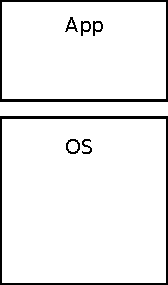
\includegraphics[width=0.4\textwidth]{res/propritary-on-os-base.pdf}
		\end{center}
	}
	\only<3|handout:0>{
		\begin{center}
			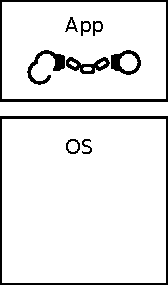
\includegraphics[width=0.4\textwidth]{res/propritary-on-os-app.pdf}
		\end{center}
	}
	\only<4|handout:0>{
		\begin{center}
			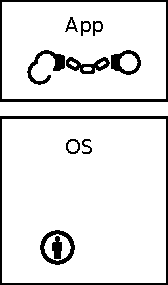
\includegraphics[width=0.4\textwidth]{res/propritary-on-os-permissive.pdf}
		\end{center}
	}
	\only<5|handout:1>{
		\begin{center}
			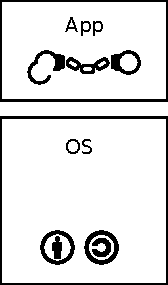
\includegraphics[width=0.4\textwidth]{res/propritary-on-os-copyleft.pdf}
		\end{center}
	}
\end{frame}
\note
{
	\begin{itemize}
		\item proprietäre Applikation auf freiem OS (z.B. Debian GNU/Linux) kein Problem
		\item Open Handcuffs: CC-0 by qubodup \url{https://openclipart.org/detail/171929/open-handcuffs}
	\end{itemize}
}

\begin{frame}{Frei mit Proprietär: Library}
	\begin{multicols}{2}
		\only<2|handout:0>{
			\begin{center}
				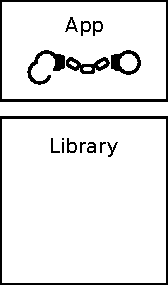
\includegraphics[width=0.4\textwidth]{res/propritary-dynamic-linking-base.pdf}
			\end{center}
		}
		\only<3|handout:0>{
			\begin{center}
				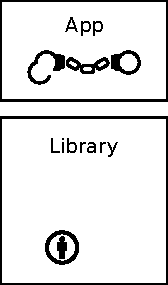
\includegraphics[width=0.4\textwidth]{res/propritary-dynamic-linking-permissive.pdf}
			\end{center}
		}
		\only<4|handout:0>{
			\begin{center}
				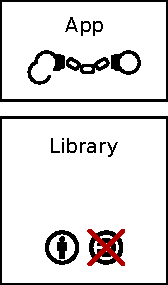
\includegraphics[width=0.4\textwidth]{res/propritary-dynamic-linking-copyleft.pdf}
			\end{center}
		}
		\only<5-|handout:1>{
			\begin{center}
				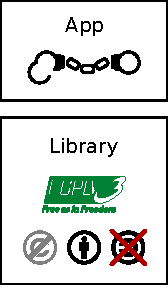
\includegraphics[width=0.4\textwidth]{res/propritary-dynamic-linking-lgpl.pdf}
			\end{center}
		}
		\pagebreak
		\only<6|handout:0>{
			\begin{center}
				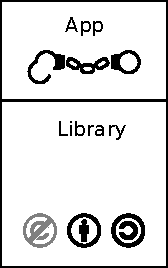
\includegraphics[width=0.4\textwidth]{res/propritary-static-linking-base.pdf}
			\end{center}
		}
		\only<7|handout:0>{
			\begin{center}
				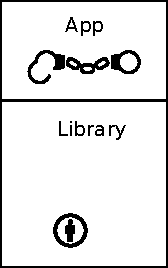
\includegraphics[width=0.4\textwidth]{res/propritary-static-linking-permissive.pdf}
			\end{center}
		}
		\only<8|handout:0>{
			\begin{center}
				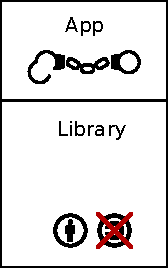
\includegraphics[width=0.4\textwidth]{res/propritary-static-linking-copyleft.pdf}
			\end{center}
		}
		\only<9-|handout:1>{
			\begin{center}
				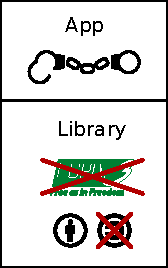
\includegraphics[width=0.4\textwidth]{res/propritary-static-linking-lgpl.pdf}
			\end{center}
		}
	\end{multicols}
\end{frame}
\note
{
	\begin{itemize}
		\item dynamisches linken nur gegen Libraries mit Public-Domain, permissiven Lizenzen oder LGPL
		\item statisches linken nur gegen Libraries mit Public-Domain oder permissiven Lizenzen
	\end{itemize}
}

\begin{frame}{Frei mit Proprietär: Code Übernahme}
	\begin{multicols}{2}
		\begin{center}
			\only<2|handout:0>{
				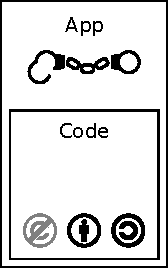
\includegraphics[width=0.4\textwidth]{res/propritary-use-code-base.pdf}
			}
			\only<3|handout:0>{
				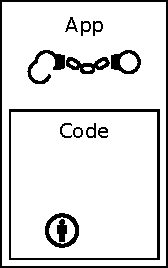
\includegraphics[width=0.4\textwidth]{res/propritary-use-code-permissive.pdf}
			}
			\only<4-|handout:1>{
				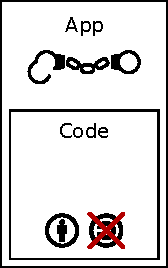
\includegraphics[width=0.4\textwidth]{res/propritary-use-code-copyleft.pdf}
			}
		\end{center}
		\pagebreak
		\only<5|handout:0>{
			\begin{center}
				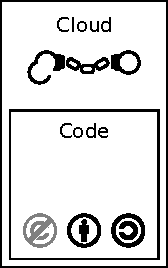
\includegraphics[width=0.4\textwidth]{res/propritary-cloud-base.pdf}
			\end{center}
		}
		\only<6|handout:0>{
			\begin{center}
				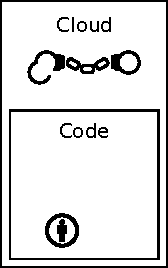
\includegraphics[width=0.4\textwidth]{res/propritary-cloud-permissive.pdf}
			\end{center}
		}
		\only<7|handout:0>{
			\begin{center}
				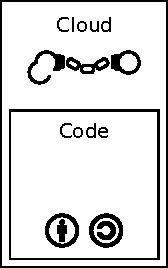
\includegraphics[width=0.4\textwidth]{res/propritary-cloud-copyleft.pdf}
			\end{center}
		}
		\only<8-|handout:1>{
			\begin{center}
				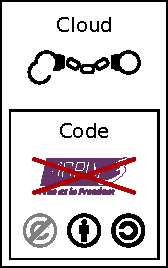
\includegraphics[width=0.4\textwidth]{res/propritary-cloud-agpl.pdf}
			\end{center}
		}
	\end{multicols}
\end{frame}
\note
{
	\begin{itemize}
		\item Verwenden in proprietärem Code: nur Public-Domain oder permissive Lizenzen
		\item Code unter Copyleft darf nicht in proprietärer Applikation verwendet werden (ausser wenn ausschliesslich intern gebraucht, dann ist es Freie Software)
		\item Wird Software als Service zur Verfügung gestellt muss der Copyleft Quelltext nicht zur Verfügung gestellt werden. Die AGPL schliesst diese Lücke. (\url{https://de.wikipedia.org/wiki/GNU\_Affero\_General\_Public\_License})
	\end{itemize}
}

\begin{frame}{Verwendung mit Freier Software}
	\pause
	\begin{itemize}
		\item Patches unter gleicher Lizenz
		\pause
		\item Lizenz Kompatibilität beachten
	\end{itemize}
	\pause
	\begin{center}
		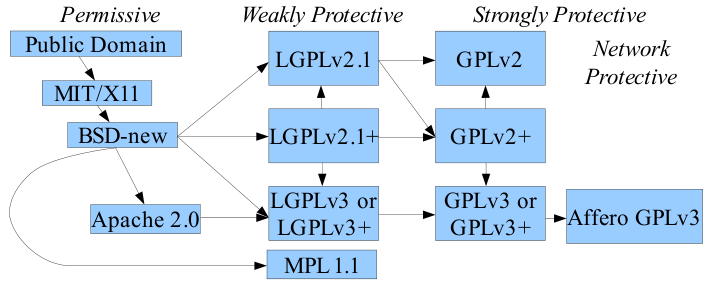
\includegraphics[width=\textwidth]{res/floss-license-compability.png}
	\end{center}
\end{frame}
\note
{
	\begin{itemize}
		\item Floss-license-slide-image.png: CC-SA 3.0 by David A. Wheeler (\url{https://commons.wikimedia.org/wiki/File:Floss-license-slide-image.png})
	\end{itemize}
}

\begin{frame}{Auswahl einer Lizenz}
	\begin{center}
		\begin{tabular}{ccc}
		\visible<2->{
\includegraphics[width=1cm]{res/PD-icon.pdf}} & \visible<4->{
\includegraphics[width=1cm]{res/by.pdf}} & \visible<6->{
\includegraphics[width=1cm]{res/copyleft.pdf}} \\ 
		\visible<2->{Public Domain} & \visible<4->{Permissiv} & \visible<6->{Copyleft} \\
		\visible<3->{
\includegraphics[width=2.8cm]{res/cc-zero.pdf}} & \visible<5->{\includegraphics[width=2.8cm]{res/mit-logo.pdf}} & \visible<7->{\includegraphics[width=2.8cm]{res/gpl-v3-logo.pdf}} \\
		\hspace{0.3\textwidth} & \hspace{0.3\textwidth} & \hspace{0.3\textwidth} \\
		\end{tabular} 
	\end{center}
	\begin{itemize}
		\visible<8->{\item \url{http://choosealicense.com/}}
	\end{itemize}
	\vspace{1cm}
\end{frame}
\note
{
	\begin{itemize}
		\item Was will man schützen?
		\item Was will man erlauben?
		\item Was will man verhindern?
	\end{itemize}
}

\begin{frame}{Deklaration der Lizenz}
	\begin{center}
		\only<2|handout:1>
		{
			\includegraphics[width=\textwidth]{res/lizenz-source.png}
		}
		\only<3|handout:2>
		{
			\includegraphics[width=\textwidth]{res/lizenz-file.png}
		}
		\only<4|handout:3>
		{
			\includegraphics[height=6cm]{res/lizenz-binary.png}
		}
	\end{center}
\end{frame}
\note
{
	\begin{itemize}
		\item im Projekt (COPYING)
		\item in den Files (Header, SPDX)
		\item in dem Binary (About Dialog, Info Option in CLI Applikationen)
		\item Keine Lizenz: Code darf nicht benutzt werden
	\end{itemize}
}

\begin{frame}{Veröffentlichen der Sourcen}
	\only<2|handout:1>{
		\begin{center}
			\makebox[\textwidth]{\includegraphics[width=0.98\paperwidth]{res/source-download.png}}
		\end{center}
	}
	\only<3|handout:2>{
		\begin{center}
			\makebox[\textwidth]{\includegraphics[width=0.98\paperwidth]{res/source-git.png}}
		\end{center}
	}
\end{frame}
\note
{
	\begin{itemize}
		\item Source des Programms muss in der gleichen Version zur Verfügung stehen
		\item Besser noch wenn Entwicklung offen und Zugriff auf Source Versionskontrolle besteht
	\end{itemize}
}

\begin{frame}{Verteidigung des eigenen Codes}
	\begin{itemize}
		\pause
		\item Dialog suchen
		\pause
		\item \url{http://gpl-violations.org}
	\end{itemize}
\end{frame}
\note
{
	\begin{itemize}
		\item \url{https://en.wikipedia.org/wiki/Gpl-violations.org}
		\item Erfolge vor Gericht
	\end{itemize}
}

\subsection{Zusammenfassung}
\subsectionframe

\begin{frame}{Zusammenfassung}
\end{frame}


% (C) Copyright 2016
% Urs Fässler, www.bitzgi.ch
% SPDX-License-Identifier: CC-BY-SA-4.0

\section{Message}

\begin{frame}
	\begin{center}
		\Huge
		wähle Lizenz\\
		deklariere Lizenz
	\end{center}
\end{frame}


\only<handout>
{
	\appendix
	\section{Backup}


\begin{frame}{Danke}
	\visible<2->{
		\begin{center}
			\includegraphics[height=2cm]{res/Question-Girl.pdf}\hcite{questionGirl}
			\includegraphics[height=2cm]{res/Question-Guy.pdf}\hcite{questionGuy}
		\end{center}
	}
%	\begin{itemize}
%		\item Slides auf \url{http://www.bitzgi.ch/presentations}
%		\item \href{https://github.com/ursfassler/embedded-gnu-linux-basics}{/embedded-gnu-linux-basics} Sourcen des Vortrags
%	\end{itemize}
	\begin{center}
		\includegraphics[width=2cm]{res/by-sa.pdf}
		\hspace{0.5cm}
		Urs Fässler
		\hspace{0.25cm}
		\includegraphics[width=2.5cm]{res/mail.pdf}
	\end{center}
\end{frame}


\begin{frame}{GPL-3}
	\todo{Übersichtlicher machen}\\
	\todo{hier oder bei der Verwendung genauer erklären?}\\
	\begin{tabular}{|c|c|c|}
		\hline 
		Can & Cannot & Must \\ 
		\hline 
		Commercial Use & Sublicense & Include Original \\ 
		\hline 
		Modify & Hold Liable & State Changes \\ 
		\hline 
		Distribute &  & Disclose Source \\ 
		\hline 
		Place Warranty &  & Include License \\ 
		\hline 
		Use Patent Claims &  & Include Copyright \\ 
		\hline 
		&  & Include Install Instructions \\ 
		\hline 
	\end{tabular} 
\end{frame}
\note
{
	\url{https://tldrlegal.com/license/gnu-general-public-license-v3-(gpl-3)}
}

\begin{frame}{FLOSS}
	\todo{Farben}\\
	\begin{center}
		\begin{tikzpicture}
		[
			node distance = 2 cm,
			box/.style = {thick, draw=black, fill=red, align=center, inner sep = 0.25cm},
			background/.style = {draw=blue},
		]
		\small

		\node (center) {};

		\visible<8->{
			\node[box, above = 2.25cm of center] (floss) {FLOSS: Free/Libre Open Source Software};
		}

		\visible<2->{
			\node[box, left = 1.75cm of center] (free) {\includegraphics[height=1cm]{res/gnu-head.pdf}};
		}
		\visible<3->{
			\node[box, above left of = free] (user) {Anwender};
			\draw (free) -- (user);
			\node[box, above right of = free] (community) {Gesellschaft};
			\draw (free) -- (community);
		}
		\visible<4->{
			\node[box, below left of = free] (ethical) {ethisch};
			\draw (free) -- (ethical);
			\node[box, below right of = free] (social) {sozial};
			\draw (free) -- (social);
		}

		\visible<5->{
			\node[box, right = 1.75cm of center] (open) {\includegraphics[height=1cm]{res/opensource.pdf}};
		}
		\visible<6->{
			\node[box, above left of = open] (developer) {Entwickler};
			\draw (open) -- (developer);
			\node[box, above right of = open] (business) {Business};
			\draw (open) -- (business);
		}
		\visible<7->{
			\node[box, below left of = open] (practical) {praktisch};
			\draw (open) -- (practical);
			\node[box, below right of = open] (pragmatic) {pragmatisch};
			\draw (open) -- (pragmatic);
		}

		\begin{pgfonlayer}{background} 
			\node[box] [fit = (floss) (free) (open) (user) (community) (ethical) (social) (developer) (business) (practical) (pragmatic)] {};
		\end{pgfonlayer}
		
		\end{tikzpicture}
	\end{center}
\end{frame}
\note
{
	\url{https://de.wikipedia.org/wiki/Freie\_Software\#Open\_Source}
	Logo Open Source Initiative: CC-SA Open Source Initiative official SVG \url{https://commons.wikimedia.org/wiki/File:Opensource.svg}
}


\begin{frame}{Werke: Creative Commons}
	\begin{center}
	\begin{tabular}{cccc}
		\includegraphics[height=1cm]{res/by.pdf}
		&
		\includegraphics[height=1cm]{res/sa.pdf}
		&
		\includegraphics[height=1cm]{res/nc.pdf}
		&
		\includegraphics[height=1cm]{res/nd.pdf}
	\\
		BY
		&
		SA
		&
		NC
		&
		ND
	\\
		Attribution
		&
		Share Alike
		&
		Non-Commercial
		&
		No Derivatives
	\\
		Frei
		&
		Frei
		&
		Unfrei
		&
		Unfrei
	\end{tabular} 
	\\
	\vspace{1cm}
	\begin{tabular}{ccc}
		\includegraphics[height=1cm]{res/cc-zero.pdf}
		&
		\includegraphics[height=1cm]{res/cc-by.pdf}
		&
		\includegraphics[height=1cm]{res/cc-by-sa.pdf}
	\\
		CC-0
		&
		CC-BY
		&
		CC-BY-SA
	\\
		Public Domain
		&
		Nachgiebig
		&
		Copyleft
	\end{tabular} 
	\\
	\vspace{1cm}
	\end{center}
\end{frame}
\note
{
	Logos sind Public Domain (\url{https://creativecommons.org/about/downloads/})
}

\begin{frame}{Best Practises in der FLOSS Community}
	\begin{itemize}
		\item release early
		\item release often
		\item offener Entwicklungsprozess
		\item einfach Kontaktierbar
		\item nett sein
	\end{itemize}
\end{frame}

\section{Literatur \& Bild-Nachweise}
\begin{frame}[allowframebreaks]{Literature}
	\tiny{
		\bibliography{literature}
	}
\end{frame}

}

\end{document}
